\documentclass[twoside]{book}

% Packages required by doxygen
\usepackage{fixltx2e}
\usepackage{calc}
\usepackage{doxygen}
\usepackage[export]{adjustbox} % also loads graphicx
\usepackage{graphicx}
\usepackage[utf8]{inputenc}
\usepackage{makeidx}
\usepackage{multicol}
\usepackage{multirow}
\PassOptionsToPackage{warn}{textcomp}
\usepackage{textcomp}
\usepackage[nointegrals]{wasysym}
\usepackage[table]{xcolor}

% Font selection
\usepackage[T1]{fontenc}
\usepackage[scaled=.90]{helvet}
\usepackage{courier}
\usepackage{amssymb}
\usepackage{sectsty}
\renewcommand{\familydefault}{\sfdefault}
\allsectionsfont{%
  \fontseries{bc}\selectfont%
  \color{darkgray}%
}
\renewcommand{\DoxyLabelFont}{%
  \fontseries{bc}\selectfont%
  \color{darkgray}%
}
\newcommand{\+}{\discretionary{\mbox{\scriptsize$\hookleftarrow$}}{}{}}

% Page & text layout
\usepackage{geometry}
\geometry{%
  a4paper,%
  top=2.5cm,%
  bottom=2.5cm,%
  left=2.5cm,%
  right=2.5cm%
}
\tolerance=750
\hfuzz=15pt
\hbadness=750
\setlength{\emergencystretch}{15pt}
\setlength{\parindent}{0cm}
\setlength{\parskip}{3ex plus 2ex minus 2ex}
\makeatletter
\renewcommand{\paragraph}{%
  \@startsection{paragraph}{4}{0ex}{-1.0ex}{1.0ex}{%
    \normalfont\normalsize\bfseries\SS@parafont%
  }%
}
\renewcommand{\subparagraph}{%
  \@startsection{subparagraph}{5}{0ex}{-1.0ex}{1.0ex}{%
    \normalfont\normalsize\bfseries\SS@subparafont%
  }%
}
\makeatother

% Headers & footers
\usepackage{fancyhdr}
\pagestyle{fancyplain}
\fancyhead[LE]{\fancyplain{}{\bfseries\thepage}}
\fancyhead[CE]{\fancyplain{}{}}
\fancyhead[RE]{\fancyplain{}{\bfseries\leftmark}}
\fancyhead[LO]{\fancyplain{}{\bfseries\rightmark}}
\fancyhead[CO]{\fancyplain{}{}}
\fancyhead[RO]{\fancyplain{}{\bfseries\thepage}}
\fancyfoot[LE]{\fancyplain{}{}}
\fancyfoot[CE]{\fancyplain{}{}}
\fancyfoot[RE]{\fancyplain{}{\bfseries\scriptsize Generated by Doxygen }}
\fancyfoot[LO]{\fancyplain{}{\bfseries\scriptsize Generated by Doxygen }}
\fancyfoot[CO]{\fancyplain{}{}}
\fancyfoot[RO]{\fancyplain{}{}}
\renewcommand{\footrulewidth}{0.4pt}
\renewcommand{\chaptermark}[1]{%
  \markboth{#1}{}%
}
\renewcommand{\sectionmark}[1]{%
  \markright{\thesection\ #1}%
}

% Indices & bibliography
\usepackage{natbib}
\usepackage[titles]{tocloft}
\setcounter{tocdepth}{3}
\setcounter{secnumdepth}{5}
\makeindex

% Hyperlinks (required, but should be loaded last)
\usepackage{ifpdf}
\ifpdf
  \usepackage[pdftex,pagebackref=true]{hyperref}
\else
  \usepackage[ps2pdf,pagebackref=true]{hyperref}
\fi
\hypersetup{%
  colorlinks=true,%
  linkcolor=blue,%
  citecolor=blue,%
  unicode%
}

% Custom commands
\newcommand{\clearemptydoublepage}{%
  \newpage{\pagestyle{empty}\cleardoublepage}%
}

\usepackage{caption}
\captionsetup{labelsep=space,justification=centering,font={bf},singlelinecheck=off,skip=4pt,position=top}

%===== C O N T E N T S =====

\begin{document}

% Titlepage & ToC
\hypersetup{pageanchor=false,
             bookmarksnumbered=true,
             pdfencoding=unicode
            }
\pagenumbering{alph}
\begin{titlepage}
\vspace*{7cm}
\begin{center}%
{\Large R\+W\+A2\+\_\+\+Group22 }\\
\vspace*{1cm}
{\large Generated by Doxygen 1.8.13}\\
\end{center}
\end{titlepage}
\clearemptydoublepage
\pagenumbering{roman}
\tableofcontents
\clearemptydoublepage
\pagenumbering{arabic}
\hypersetup{pageanchor=true}

%--- Begin generated contents ---
\chapter{Maze search algorithm}
\label{index}\hypertarget{index}{}This project consists of searching a path in a maze and then task a mouse (robot) to follow the path.
\begin{DoxyItemize}
\item \hyperlink{searchingPathPage}{Searching a path}
\item \hyperlink{followingPathPage}{Following a path} 
\end{DoxyItemize}
\chapter{Searching a path}
\label{searching_path_page}
\Hypertarget{searching_path_page}
The search algorithm used for searching a path in a maze relies on the depth-\/first search (D\+FS) approach. This algorithm is implemented in \hyperlink{classrwa2_1_1_mouse_a789be287a432bafc903c97396a014d7d}{rwa2\+::\+Mouse\+::search\+\_\+maze()} 
\chapter{Following a path}
\label{following_path_page}
\Hypertarget{following_path_page}
To follow a path generated by D\+FS, methods from the class \hyperlink{class_a_p_i}{A\+PI} (\hyperlink{api_8h}{api/api.\+h}) must be used to interact with the micromouse simulator.
\begin{DoxyItemize}
\item Methods of the \hyperlink{class_a_p_i}{A\+PI} class are documented \href{https://github.com/mackorone/mms#summary}{\tt here}. 
\end{DoxyItemize}
\chapter{Class Index}
\section{Class List}
Here are the classes, structs, unions and interfaces with brief descriptions\+:\begin{DoxyCompactList}
\item\contentsline{section}{\hyperlink{class_a_p_i}{A\+PI} }{\pageref{class_a_p_i}}{}
\item\contentsline{section}{\hyperlink{classrwa2_1_1_mouse}{rwa2\+::\+Mouse} \\*This class is used to compute a path and execute the path }{\pageref{classrwa2_1_1_mouse}}{}
\item\contentsline{section}{\hyperlink{classrwa2_1_1_node}{rwa2\+::\+Node} \\*Class to represent a node (cell) in a maze }{\pageref{classrwa2_1_1_node}}{}
\end{DoxyCompactList}

\chapter{File Index}
\section{File List}
Here is a list of all documented files with brief descriptions\+:\begin{DoxyCompactList}
\item\contentsline{section}{include/api/\hyperlink{api_8h}{api.\+h} \\*This file is copied from the example downloaded from github }{\pageref{api_8h}}{}
\item\contentsline{section}{include/mouse/\hyperlink{mouse_8h}{mouse.\+h} \\*The file contains the Mouse class }{\pageref{mouse_8h}}{}
\item\contentsline{section}{include/node/\hyperlink{node_8h}{node.\+h} \\*This file contains a class to represent a node in a maze }{\pageref{node_8h}}{}
\item\contentsline{section}{include/util/\hyperlink{util_8h}{util.\+h} \\*Components used by multiple classes but not required to be a class member can be placed in this file }{\pageref{util_8h}}{}
\end{DoxyCompactList}

\chapter{Class Documentation}
\hypertarget{class_a_p_i}{}\section{A\+PI Class Reference}
\label{class_a_p_i}\index{A\+PI@{A\+PI}}
\subsection*{Static Public Member Functions}
\begin{DoxyCompactItemize}
\item 
\mbox{\Hypertarget{class_a_p_i_aad4f60e45d012af3985946b3a3bd561c}\label{class_a_p_i_aad4f60e45d012af3985946b3a3bd561c}} 
static int {\bfseries maze\+Width} ()
\item 
\mbox{\Hypertarget{class_a_p_i_ae356a8b8b3090ec8e5e66fb9d7e827a6}\label{class_a_p_i_ae356a8b8b3090ec8e5e66fb9d7e827a6}} 
static int {\bfseries maze\+Height} ()
\item 
\mbox{\Hypertarget{class_a_p_i_a3452beb4232e7960ffdb8c0d4a1f0d30}\label{class_a_p_i_a3452beb4232e7960ffdb8c0d4a1f0d30}} 
static bool {\bfseries wall\+Front} ()
\item 
\mbox{\Hypertarget{class_a_p_i_acdc812c3acadeb2890691e6c95a89816}\label{class_a_p_i_acdc812c3acadeb2890691e6c95a89816}} 
static bool {\bfseries wall\+Right} ()
\item 
\mbox{\Hypertarget{class_a_p_i_a43b1e7f9b91aba577078af681c7807b3}\label{class_a_p_i_a43b1e7f9b91aba577078af681c7807b3}} 
static bool {\bfseries wall\+Left} ()
\item 
\mbox{\Hypertarget{class_a_p_i_a25ace37c644938df32f6dae69abfe052}\label{class_a_p_i_a25ace37c644938df32f6dae69abfe052}} 
static void {\bfseries move\+Forward} (int distance=1)
\item 
\mbox{\Hypertarget{class_a_p_i_a4b5aaf5e3e061474d84191ab9ee05d63}\label{class_a_p_i_a4b5aaf5e3e061474d84191ab9ee05d63}} 
static void {\bfseries turn\+Right} ()
\item 
\mbox{\Hypertarget{class_a_p_i_af04ee9209026f2a6e1c502e6c900573f}\label{class_a_p_i_af04ee9209026f2a6e1c502e6c900573f}} 
static void {\bfseries turn\+Left} ()
\item 
\mbox{\Hypertarget{class_a_p_i_a9b0b04cf1cfc62ae6f5eef1ac1729eb2}\label{class_a_p_i_a9b0b04cf1cfc62ae6f5eef1ac1729eb2}} 
static void {\bfseries set\+Wall} (int x, int y, char \hyperlink{util_8h_a99f26e6ee9fcd62f75203b5402df8098}{direction})
\item 
\mbox{\Hypertarget{class_a_p_i_a3178d408a832d81500847ca62ce1f509}\label{class_a_p_i_a3178d408a832d81500847ca62ce1f509}} 
static void {\bfseries clear\+Wall} (int x, int y, char \hyperlink{util_8h_a99f26e6ee9fcd62f75203b5402df8098}{direction})
\item 
\mbox{\Hypertarget{class_a_p_i_aee5aaa673b406ddaab3310fcb3a51d83}\label{class_a_p_i_aee5aaa673b406ddaab3310fcb3a51d83}} 
static void {\bfseries set\+Color} (int x, int y, char color)
\item 
\mbox{\Hypertarget{class_a_p_i_ae5c04edd8e44f455ac6bf8a19c2ba282}\label{class_a_p_i_ae5c04edd8e44f455ac6bf8a19c2ba282}} 
static void {\bfseries clear\+Color} (int x, int y)
\item 
\mbox{\Hypertarget{class_a_p_i_a26cc8c35d6c492fc782647b7e347525e}\label{class_a_p_i_a26cc8c35d6c492fc782647b7e347525e}} 
static void {\bfseries clear\+All\+Color} ()
\item 
\mbox{\Hypertarget{class_a_p_i_a25a489520b0b69b7a0b1870cf350f654}\label{class_a_p_i_a25a489520b0b69b7a0b1870cf350f654}} 
static void {\bfseries set\+Text} (int x, int y, const std\+::string \&text)
\item 
\mbox{\Hypertarget{class_a_p_i_a0937e059fff7d9543187765500fa4968}\label{class_a_p_i_a0937e059fff7d9543187765500fa4968}} 
static void {\bfseries clear\+Text} (int x, int y)
\item 
\mbox{\Hypertarget{class_a_p_i_a212ef41a4d954a80cd08f462fdb9f631}\label{class_a_p_i_a212ef41a4d954a80cd08f462fdb9f631}} 
static void {\bfseries clear\+All\+Text} ()
\item 
\mbox{\Hypertarget{class_a_p_i_ab754e11300491d9efee2da2eda368d93}\label{class_a_p_i_ab754e11300491d9efee2da2eda368d93}} 
static bool {\bfseries was\+Reset} ()
\item 
\mbox{\Hypertarget{class_a_p_i_a3e6a76df2da89bd7f7fc72a96e0a9094}\label{class_a_p_i_a3e6a76df2da89bd7f7fc72a96e0a9094}} 
static void {\bfseries ack\+Reset} ()
\end{DoxyCompactItemize}


The documentation for this class was generated from the following files\+:\begin{DoxyCompactItemize}
\item 
include/api/\hyperlink{api_8h}{api.\+h}\item 
src/api.\+cpp\end{DoxyCompactItemize}

\hypertarget{classrwa2_1_1_mouse}{}\section{rwa2\+:\+:Mouse Class Reference}
\label{classrwa2_1_1_mouse}\index{rwa2\+::\+Mouse@{rwa2\+::\+Mouse}}


This class is used to compute a path and execute the path.  




{\ttfamily \#include $<$mouse.\+h$>$}

\subsection*{Public Member Functions}
\begin{DoxyCompactItemize}
\item 
\hyperlink{classrwa2_1_1_mouse_a048dffae3aaa3a6ddc2c6cc4741a097c}{Mouse} ()
\begin{DoxyCompactList}\small\item\em Construct a new Micro\+Mouse object. \end{DoxyCompactList}\item 
\mbox{\Hypertarget{classrwa2_1_1_mouse_abbcc99c41fd073426fdfd790f947956e}\label{classrwa2_1_1_mouse_abbcc99c41fd073426fdfd790f947956e}} 
void {\bfseries display\+\_\+walls} ()
\item 
bool \hyperlink{classrwa2_1_1_mouse_a789be287a432bafc903c97396a014d7d}{search\+\_\+maze} ()
\begin{DoxyCompactList}\small\item\em Implement D\+FS to compute a path between 2 nodes in a maze. \end{DoxyCompactList}\item 
bool \hyperlink{classrwa2_1_1_mouse_a35873f1fd775399f6506a1da415a8da9}{check\+\_\+validity} (int, int, int)
\begin{DoxyCompactList}\small\item\em Check whether travelling to the next node is possible. \end{DoxyCompactList}\item 
bool \hyperlink{classrwa2_1_1_mouse_a760964c393cf8861429d2e02aba4f033}{check\+\_\+list} (std\+::array$<$ int, 2 $>$, std\+::vector$<$ std\+::array$<$ int, 2 $>$$>$)
\begin{DoxyCompactList}\small\item\em Check if the input array is part of the given list. \end{DoxyCompactList}\item 
\mbox{\Hypertarget{classrwa2_1_1_mouse_ac33256110d3f1a3d2c1f0498898fc334}\label{classrwa2_1_1_mouse_ac33256110d3f1a3d2c1f0498898fc334}} 
void \hyperlink{classrwa2_1_1_mouse_ac33256110d3f1a3d2c1f0498898fc334}{move\+\_\+mouse} ()
\begin{DoxyCompactList}\small\item\em Move the mouse in the simulator. \end{DoxyCompactList}\item 
\mbox{\Hypertarget{classrwa2_1_1_mouse_ad9a06996a95ce3b02acc0a266e0cfe6c}\label{classrwa2_1_1_mouse_ad9a06996a95ce3b02acc0a266e0cfe6c}} 
void \hyperlink{classrwa2_1_1_mouse_ad9a06996a95ce3b02acc0a266e0cfe6c}{check\+\_\+walls} ()
\begin{DoxyCompactList}\small\item\em Check whether there are walls around the current node. \end{DoxyCompactList}\item 
std\+::array$<$ int, 2 $>$ \hyperlink{classrwa2_1_1_mouse_a204d9d2ff255e82885ef3541c77fb0fb}{get\+\_\+goal} ()
\begin{DoxyCompactList}\small\item\em Get the goal. \end{DoxyCompactList}\item 
\mbox{\Hypertarget{classrwa2_1_1_mouse_a81a6dc8ebe05e7d75b7f3fb5537be739}\label{classrwa2_1_1_mouse_a81a6dc8ebe05e7d75b7f3fb5537be739}} 
void \hyperlink{classrwa2_1_1_mouse_a81a6dc8ebe05e7d75b7f3fb5537be739}{set\+\_\+goal} (std\+::array$<$ int, 2 $>$)
\begin{DoxyCompactList}\small\item\em Set the goal object. \end{DoxyCompactList}\item 
bool \hyperlink{classrwa2_1_1_mouse_a67629e9752358e8a0207e9517e5c904d}{get\+\_\+break\+\_\+flag} ()
\begin{DoxyCompactList}\small\item\em Get the break flag condition. \end{DoxyCompactList}\item 
\mbox{\Hypertarget{classrwa2_1_1_mouse_abb5990dd5f19cd8453011199ebd3240b}\label{classrwa2_1_1_mouse_abb5990dd5f19cd8453011199ebd3240b}} 
void \hyperlink{classrwa2_1_1_mouse_abb5990dd5f19cd8453011199ebd3240b}{set\+\_\+break\+\_\+flag} (bool)
\begin{DoxyCompactList}\small\item\em Change the value of the break flag condition. \end{DoxyCompactList}\item 
\mbox{\Hypertarget{classrwa2_1_1_mouse_a24410ed49bebf1570e466aa5151a6ad3}\label{classrwa2_1_1_mouse_a24410ed49bebf1570e466aa5151a6ad3}} 
void \hyperlink{classrwa2_1_1_mouse_a24410ed49bebf1570e466aa5151a6ad3}{clear\+\_\+list} ()
\begin{DoxyCompactList}\small\item\em Clear the list of visited nodes. \end{DoxyCompactList}\item 
std\+::stack$<$ std\+::array$<$ int, 2 $>$ $>$ \hyperlink{classrwa2_1_1_mouse_a809c9a41608037e6af0910765fe6fa06}{get\+\_\+stack} ()
\begin{DoxyCompactList}\small\item\em Get the stack. \end{DoxyCompactList}\item 
std\+::stack$<$ std\+::array$<$ int, 2 $>$ $>$ \hyperlink{classrwa2_1_1_mouse_aa6d86495a913a892ae279016d9e1181d}{get\+\_\+inv\+\_\+stack} ()
\begin{DoxyCompactList}\small\item\em Get the inverted stack. \end{DoxyCompactList}\item 
\mbox{\Hypertarget{classrwa2_1_1_mouse_ab9bf8e2e4ac74c9b4294d8e55b6d3015}\label{classrwa2_1_1_mouse_ab9bf8e2e4ac74c9b4294d8e55b6d3015}} 
void \hyperlink{classrwa2_1_1_mouse_ab9bf8e2e4ac74c9b4294d8e55b6d3015}{push\+\_\+inv\+\_\+stack} (std\+::array$<$ int, 2 $>$)
\begin{DoxyCompactList}\small\item\em Method to push new element in stack. \end{DoxyCompactList}\item 
\mbox{\Hypertarget{classrwa2_1_1_mouse_a0167912e328d9bae9d755f6b3498cddf}\label{classrwa2_1_1_mouse_a0167912e328d9bae9d755f6b3498cddf}} 
void \hyperlink{classrwa2_1_1_mouse_a0167912e328d9bae9d755f6b3498cddf}{pop\+\_\+stack} ()
\begin{DoxyCompactList}\small\item\em Method to pop the stack. \end{DoxyCompactList}\item 
\mbox{\Hypertarget{classrwa2_1_1_mouse_affb37079cca281108a63ec5ec73f63aa}\label{classrwa2_1_1_mouse_affb37079cca281108a63ec5ec73f63aa}} 
void \hyperlink{classrwa2_1_1_mouse_affb37079cca281108a63ec5ec73f63aa}{pop\+\_\+inv\+\_\+stack} ()
\begin{DoxyCompactList}\small\item\em Method to pop the inverted stack. \end{DoxyCompactList}\end{DoxyCompactItemize}


\subsection{Detailed Description}
This class is used to compute a path and execute the path. 

\subsection{Constructor \& Destructor Documentation}
\mbox{\Hypertarget{classrwa2_1_1_mouse_a048dffae3aaa3a6ddc2c6cc4741a097c}\label{classrwa2_1_1_mouse_a048dffae3aaa3a6ddc2c6cc4741a097c}} 
\index{rwa2\+::\+Mouse@{rwa2\+::\+Mouse}!Mouse@{Mouse}}
\index{Mouse@{Mouse}!rwa2\+::\+Mouse@{rwa2\+::\+Mouse}}
\subsubsection{\texorpdfstring{Mouse()}{Mouse()}}
{\footnotesize\ttfamily rwa2\+::\+Mouse\+::\+Mouse (\begin{DoxyParamCaption}{ }\end{DoxyParamCaption})\hspace{0.3cm}{\ttfamily [inline]}}



Construct a new Micro\+Mouse object. 

The robot is always at (0,0) and facing N\+O\+R\+TH when the simulator starts Here is the call graph for this function\+:\nopagebreak
\begin{figure}[H]
\begin{center}
\leavevmode
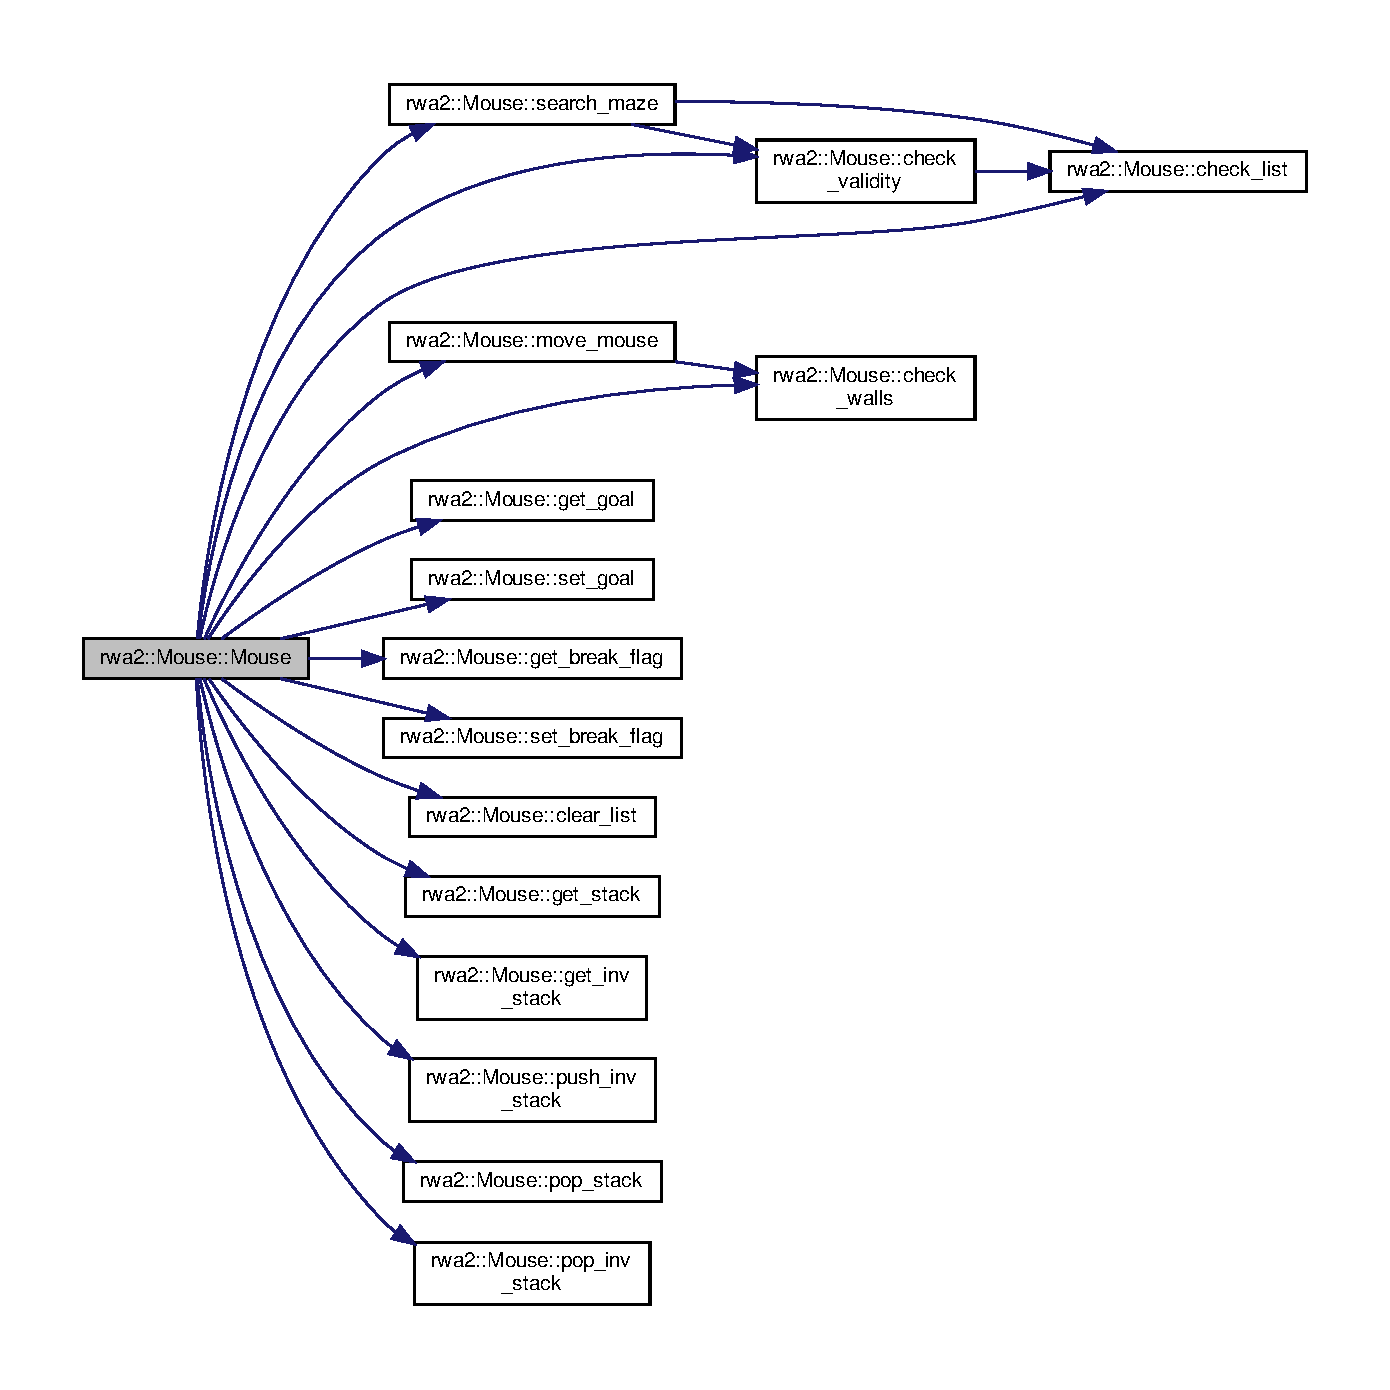
\includegraphics[width=350pt]{classrwa2_1_1_mouse_a048dffae3aaa3a6ddc2c6cc4741a097c_cgraph}
\end{center}
\end{figure}


\subsection{Member Function Documentation}
\mbox{\Hypertarget{classrwa2_1_1_mouse_a760964c393cf8861429d2e02aba4f033}\label{classrwa2_1_1_mouse_a760964c393cf8861429d2e02aba4f033}} 
\index{rwa2\+::\+Mouse@{rwa2\+::\+Mouse}!check\+\_\+list@{check\+\_\+list}}
\index{check\+\_\+list@{check\+\_\+list}!rwa2\+::\+Mouse@{rwa2\+::\+Mouse}}
\subsubsection{\texorpdfstring{check\+\_\+list()}{check\_list()}}
{\footnotesize\ttfamily bool rwa2\+::\+Mouse\+::check\+\_\+list (\begin{DoxyParamCaption}\item[{std\+::array$<$ int, 2 $>$}]{p,  }\item[{std\+::vector$<$ std\+::array$<$ int, 2 $>$$>$}]{v }\end{DoxyParamCaption})}



Check if the input array is part of the given list. 

\begin{DoxyReturn}{Returns}
true 

false 
\end{DoxyReturn}
\mbox{\Hypertarget{classrwa2_1_1_mouse_a35873f1fd775399f6506a1da415a8da9}\label{classrwa2_1_1_mouse_a35873f1fd775399f6506a1da415a8da9}} 
\index{rwa2\+::\+Mouse@{rwa2\+::\+Mouse}!check\+\_\+validity@{check\+\_\+validity}}
\index{check\+\_\+validity@{check\+\_\+validity}!rwa2\+::\+Mouse@{rwa2\+::\+Mouse}}
\subsubsection{\texorpdfstring{check\+\_\+validity()}{check\_validity()}}
{\footnotesize\ttfamily bool rwa2\+::\+Mouse\+::check\+\_\+validity (\begin{DoxyParamCaption}\item[{int}]{dir,  }\item[{int}]{x,  }\item[{int}]{y }\end{DoxyParamCaption})}



Check whether travelling to the next node is possible. 

\begin{DoxyReturn}{Returns}
true 

false 
\end{DoxyReturn}
Here is the call graph for this function\+:\nopagebreak
\begin{figure}[H]
\begin{center}
\leavevmode
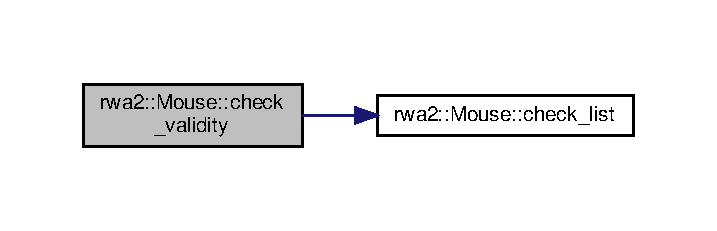
\includegraphics[width=344pt]{classrwa2_1_1_mouse_a35873f1fd775399f6506a1da415a8da9_cgraph}
\end{center}
\end{figure}
\mbox{\Hypertarget{classrwa2_1_1_mouse_a67629e9752358e8a0207e9517e5c904d}\label{classrwa2_1_1_mouse_a67629e9752358e8a0207e9517e5c904d}} 
\index{rwa2\+::\+Mouse@{rwa2\+::\+Mouse}!get\+\_\+break\+\_\+flag@{get\+\_\+break\+\_\+flag}}
\index{get\+\_\+break\+\_\+flag@{get\+\_\+break\+\_\+flag}!rwa2\+::\+Mouse@{rwa2\+::\+Mouse}}
\subsubsection{\texorpdfstring{get\+\_\+break\+\_\+flag()}{get\_break\_flag()}}
{\footnotesize\ttfamily bool rwa2\+::\+Mouse\+::get\+\_\+break\+\_\+flag (\begin{DoxyParamCaption}{ }\end{DoxyParamCaption})}



Get the break flag condition. 

\begin{DoxyReturn}{Returns}
true 

false 
\end{DoxyReturn}
\mbox{\Hypertarget{classrwa2_1_1_mouse_a204d9d2ff255e82885ef3541c77fb0fb}\label{classrwa2_1_1_mouse_a204d9d2ff255e82885ef3541c77fb0fb}} 
\index{rwa2\+::\+Mouse@{rwa2\+::\+Mouse}!get\+\_\+goal@{get\+\_\+goal}}
\index{get\+\_\+goal@{get\+\_\+goal}!rwa2\+::\+Mouse@{rwa2\+::\+Mouse}}
\subsubsection{\texorpdfstring{get\+\_\+goal()}{get\_goal()}}
{\footnotesize\ttfamily std\+::array$<$ int, 2 $>$ rwa2\+::\+Mouse\+::get\+\_\+goal (\begin{DoxyParamCaption}{ }\end{DoxyParamCaption})}



Get the goal. 

\begin{DoxyReturn}{Returns}
std\+::array$<$int,2$>$ 
\end{DoxyReturn}
\mbox{\Hypertarget{classrwa2_1_1_mouse_aa6d86495a913a892ae279016d9e1181d}\label{classrwa2_1_1_mouse_aa6d86495a913a892ae279016d9e1181d}} 
\index{rwa2\+::\+Mouse@{rwa2\+::\+Mouse}!get\+\_\+inv\+\_\+stack@{get\+\_\+inv\+\_\+stack}}
\index{get\+\_\+inv\+\_\+stack@{get\+\_\+inv\+\_\+stack}!rwa2\+::\+Mouse@{rwa2\+::\+Mouse}}
\subsubsection{\texorpdfstring{get\+\_\+inv\+\_\+stack()}{get\_inv\_stack()}}
{\footnotesize\ttfamily std\+::stack$<$ std\+::array$<$ int, 2 $>$ $>$ rwa2\+::\+Mouse\+::get\+\_\+inv\+\_\+stack (\begin{DoxyParamCaption}{ }\end{DoxyParamCaption})}



Get the inverted stack. 

\begin{DoxyReturn}{Returns}
std\+::stack$<$std\+::array$<$int, 2$>$$>$ 
\end{DoxyReturn}
\mbox{\Hypertarget{classrwa2_1_1_mouse_a809c9a41608037e6af0910765fe6fa06}\label{classrwa2_1_1_mouse_a809c9a41608037e6af0910765fe6fa06}} 
\index{rwa2\+::\+Mouse@{rwa2\+::\+Mouse}!get\+\_\+stack@{get\+\_\+stack}}
\index{get\+\_\+stack@{get\+\_\+stack}!rwa2\+::\+Mouse@{rwa2\+::\+Mouse}}
\subsubsection{\texorpdfstring{get\+\_\+stack()}{get\_stack()}}
{\footnotesize\ttfamily std\+::stack$<$ std\+::array$<$ int, 2 $>$ $>$ rwa2\+::\+Mouse\+::get\+\_\+stack (\begin{DoxyParamCaption}{ }\end{DoxyParamCaption})}



Get the stack. 

\begin{DoxyReturn}{Returns}
std\+::stack$<$std\+::array$<$int, 2$>$$>$ 
\end{DoxyReturn}
\mbox{\Hypertarget{classrwa2_1_1_mouse_a789be287a432bafc903c97396a014d7d}\label{classrwa2_1_1_mouse_a789be287a432bafc903c97396a014d7d}} 
\index{rwa2\+::\+Mouse@{rwa2\+::\+Mouse}!search\+\_\+maze@{search\+\_\+maze}}
\index{search\+\_\+maze@{search\+\_\+maze}!rwa2\+::\+Mouse@{rwa2\+::\+Mouse}}
\subsubsection{\texorpdfstring{search\+\_\+maze()}{search\_maze()}}
{\footnotesize\ttfamily bool rwa2\+::\+Mouse\+::search\+\_\+maze (\begin{DoxyParamCaption}{ }\end{DoxyParamCaption})}



Implement D\+FS to compute a path between 2 nodes in a maze. 

\begin{DoxyReturn}{Returns}
true A path is found 

false A path is not found 
\end{DoxyReturn}
Here is the call graph for this function\+:\nopagebreak
\begin{figure}[H]
\begin{center}
\leavevmode
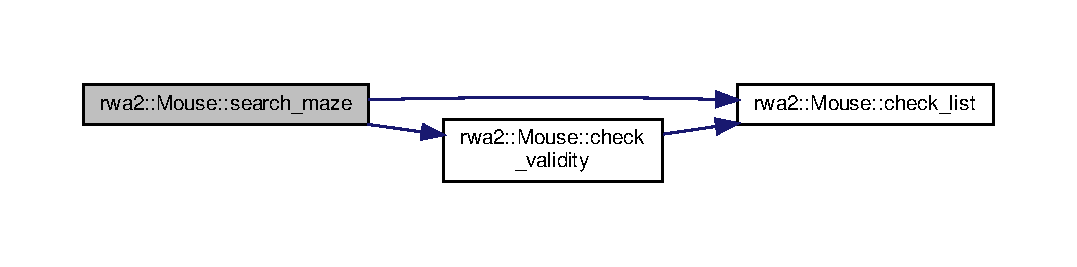
\includegraphics[width=350pt]{classrwa2_1_1_mouse_a789be287a432bafc903c97396a014d7d_cgraph}
\end{center}
\end{figure}


The documentation for this class was generated from the following files\+:\begin{DoxyCompactItemize}
\item 
include/mouse/\hyperlink{mouse_8h}{mouse.\+h}\item 
src/mouse.\+cpp\end{DoxyCompactItemize}

\hypertarget{classrwa2_1_1_node}{}\section{rwa2\+:\+:Node Class Reference}
\label{classrwa2_1_1_node}\index{rwa2\+::\+Node@{rwa2\+::\+Node}}


Class to represent a node (cell) in a maze.  




{\ttfamily \#include $<$node.\+h$>$}

\subsection*{Public Member Functions}
\begin{DoxyCompactItemize}
\item 
void \hyperlink{classrwa2_1_1_node_a9e887221d02616392f572dd4018b71ed}{set\+\_\+wall} (int \hyperlink{util_8h_a99f26e6ee9fcd62f75203b5402df8098}{direction}, bool \hyperlink{classrwa2_1_1_node_acd6ab64157b7b60bea708ddb52ddb1a8}{is\+\_\+wall})
\begin{DoxyCompactList}\small\item\em Set the wall of a cell. \end{DoxyCompactList}\item 
bool \hyperlink{classrwa2_1_1_node_acd6ab64157b7b60bea708ddb52ddb1a8}{is\+\_\+wall} (int \hyperlink{util_8h_a99f26e6ee9fcd62f75203b5402df8098}{direction}) const
\begin{DoxyCompactList}\small\item\em Return whether or not there is a wall in a cell. \end{DoxyCompactList}\item 
int \hyperlink{classrwa2_1_1_node_a6057b0b97f6b815a57aad534cd021674}{compute\+\_\+number\+\_\+of\+\_\+walls} () const
\begin{DoxyCompactList}\small\item\em Compute the number of walls surrounding a node. \end{DoxyCompactList}\end{DoxyCompactItemize}


\subsection{Detailed Description}
Class to represent a node (cell) in a maze. 

A node is just a space delimited by 4 walls 

\subsection{Member Function Documentation}
\mbox{\Hypertarget{classrwa2_1_1_node_a6057b0b97f6b815a57aad534cd021674}\label{classrwa2_1_1_node_a6057b0b97f6b815a57aad534cd021674}} 
\index{rwa2\+::\+Node@{rwa2\+::\+Node}!compute\+\_\+number\+\_\+of\+\_\+walls@{compute\+\_\+number\+\_\+of\+\_\+walls}}
\index{compute\+\_\+number\+\_\+of\+\_\+walls@{compute\+\_\+number\+\_\+of\+\_\+walls}!rwa2\+::\+Node@{rwa2\+::\+Node}}
\subsubsection{\texorpdfstring{compute\+\_\+number\+\_\+of\+\_\+walls()}{compute\_number\_of\_walls()}}
{\footnotesize\ttfamily int rwa2\+::\+Node\+::compute\+\_\+number\+\_\+of\+\_\+walls (\begin{DoxyParamCaption}{ }\end{DoxyParamCaption}) const}



Compute the number of walls surrounding a node. 

\begin{DoxyReturn}{Returns}
int Number of walls surrounding a node 
\end{DoxyReturn}
Here is the call graph for this function\+:\nopagebreak
\begin{figure}[H]
\begin{center}
\leavevmode
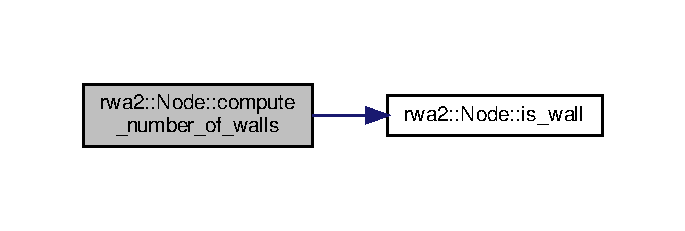
\includegraphics[width=329pt]{classrwa2_1_1_node_a6057b0b97f6b815a57aad534cd021674_cgraph}
\end{center}
\end{figure}
\mbox{\Hypertarget{classrwa2_1_1_node_acd6ab64157b7b60bea708ddb52ddb1a8}\label{classrwa2_1_1_node_acd6ab64157b7b60bea708ddb52ddb1a8}} 
\index{rwa2\+::\+Node@{rwa2\+::\+Node}!is\+\_\+wall@{is\+\_\+wall}}
\index{is\+\_\+wall@{is\+\_\+wall}!rwa2\+::\+Node@{rwa2\+::\+Node}}
\subsubsection{\texorpdfstring{is\+\_\+wall()}{is\_wall()}}
{\footnotesize\ttfamily bool rwa2\+::\+Node\+::is\+\_\+wall (\begin{DoxyParamCaption}\item[{int}]{direction }\end{DoxyParamCaption}) const}



Return whether or not there is a wall in a cell. 


\begin{DoxyParams}{Parameters}
{\em direction} & Direction to set for wall (N\+O\+R\+TH, E\+A\+ST, S\+O\+U\+TH, or W\+E\+ST) \\
\hline
\end{DoxyParams}
\begin{DoxyReturn}{Returns}
true There is a wall in the given direction in the cell 

false There is no wall in the given direction in the cell 
\end{DoxyReturn}
\mbox{\Hypertarget{classrwa2_1_1_node_a9e887221d02616392f572dd4018b71ed}\label{classrwa2_1_1_node_a9e887221d02616392f572dd4018b71ed}} 
\index{rwa2\+::\+Node@{rwa2\+::\+Node}!set\+\_\+wall@{set\+\_\+wall}}
\index{set\+\_\+wall@{set\+\_\+wall}!rwa2\+::\+Node@{rwa2\+::\+Node}}
\subsubsection{\texorpdfstring{set\+\_\+wall()}{set\_wall()}}
{\footnotesize\ttfamily void rwa2\+::\+Node\+::set\+\_\+wall (\begin{DoxyParamCaption}\item[{int}]{direction,  }\item[{bool}]{is\+\_\+wall }\end{DoxyParamCaption})}



Set the wall of a cell. 


\begin{DoxyParams}{Parameters}
{\em direction} & N\+O\+R\+TH, E\+A\+ST, S\+O\+U\+TH, or W\+E\+ST \\
\hline
{\em is\+\_\+wall} & true if there is a wall, otherwise false \\
\hline
\end{DoxyParams}
Here is the call graph for this function\+:\nopagebreak
\begin{figure}[H]
\begin{center}
\leavevmode
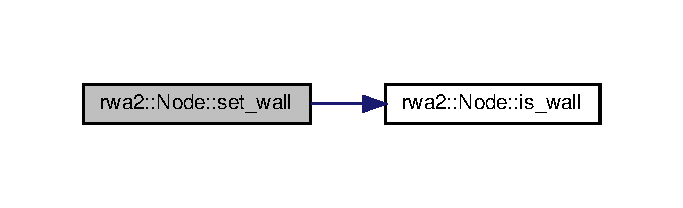
\includegraphics[width=328pt]{classrwa2_1_1_node_a9e887221d02616392f572dd4018b71ed_cgraph}
\end{center}
\end{figure}


The documentation for this class was generated from the following files\+:\begin{DoxyCompactItemize}
\item 
include/node/\hyperlink{node_8h}{node.\+h}\item 
src/node.\+cpp\end{DoxyCompactItemize}

\chapter{File Documentation}
\hypertarget{api_8h}{}\section{include/api/api.h File Reference}
\label{api_8h}\index{include/api/api.\+h@{include/api/api.\+h}}


This file is copied from the example downloaded from github.  


{\ttfamily \#include $<$string$>$}\newline
Include dependency graph for api.\+h\+:\nopagebreak
\begin{figure}[H]
\begin{center}
\leavevmode
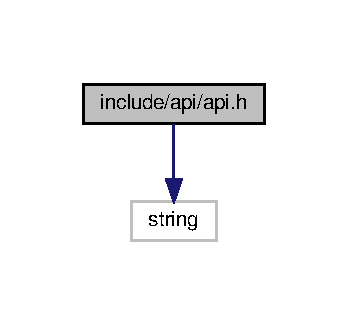
\includegraphics[width=167pt]{api_8h__incl}
\end{center}
\end{figure}
\subsection*{Classes}
\begin{DoxyCompactItemize}
\item 
class \hyperlink{class_a_p_i}{A\+PI}
\end{DoxyCompactItemize}


\subsection{Detailed Description}
This file is copied from the example downloaded from github. 

\begin{DoxyAuthor}{Author}
Zeid Kootbally (\href{mailto:zeidk@umd.edu}{\tt zeidk@umd.\+edu}) This file consists of all the methods to interact with the simulator 
\end{DoxyAuthor}
\begin{DoxyVersion}{Version}
0.\+1 
\end{DoxyVersion}
\begin{DoxyDate}{Date}
2021-\/10-\/24
\end{DoxyDate}
\begin{DoxyCopyright}{Copyright}
Copyright (c) 2021 
\end{DoxyCopyright}

\hypertarget{mouse_8h}{}\section{include/mouse/mouse.h File Reference}
\label{mouse_8h}\index{include/mouse/mouse.\+h@{include/mouse/mouse.\+h}}


The file contains the Mouse class.  


{\ttfamily \#include \char`\"{}../node/node.\+h\char`\"{}}\newline
{\ttfamily \#include \char`\"{}../util/util.\+h\char`\"{}}\newline
{\ttfamily \#include $<$array$>$}\newline
{\ttfamily \#include $<$vector$>$}\newline
{\ttfamily \#include $<$stack$>$}\newline
Include dependency graph for mouse.\+h\+:\nopagebreak
\begin{figure}[H]
\begin{center}
\leavevmode
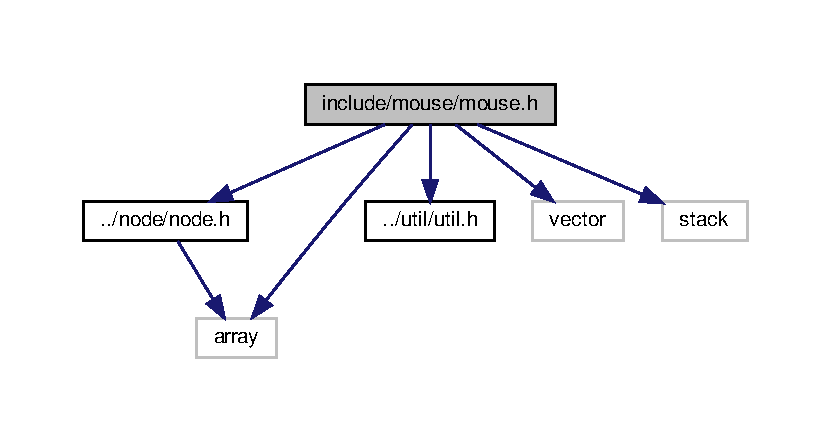
\includegraphics[width=350pt]{mouse_8h__incl}
\end{center}
\end{figure}
\subsection*{Classes}
\begin{DoxyCompactItemize}
\item 
class \hyperlink{classrwa2_1_1_mouse}{rwa2\+::\+Mouse}
\begin{DoxyCompactList}\small\item\em This class is used to compute a path and execute the path. \end{DoxyCompactList}\end{DoxyCompactItemize}


\subsection{Detailed Description}
The file contains the Mouse class. 

\begin{DoxyAuthor}{Author}
Ninad Harishchandrakar (\href{mailto:ninadh@umd.edu}{\tt ninadh@umd.\+edu}) 
\end{DoxyAuthor}
\begin{DoxyVersion}{Version}
0.\+1 
\end{DoxyVersion}
\begin{DoxyDate}{Date}
2021-\/11-\/15
\end{DoxyDate}
\begin{DoxyCopyright}{Copyright}
Copyright (c) 2021 
\end{DoxyCopyright}

\hypertarget{node_8h}{}\section{include/node/node.h File Reference}
\label{node_8h}\index{include/node/node.\+h@{include/node/node.\+h}}


This file contains a class to represent a node in a maze.  


{\ttfamily \#include $<$array$>$}\newline
Include dependency graph for node.\+h\+:\nopagebreak
\begin{figure}[H]
\begin{center}
\leavevmode
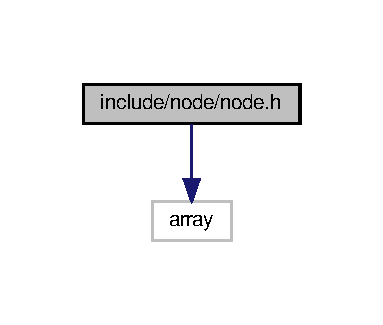
\includegraphics[width=184pt]{node_8h__incl}
\end{center}
\end{figure}
This graph shows which files directly or indirectly include this file\+:\nopagebreak
\begin{figure}[H]
\begin{center}
\leavevmode
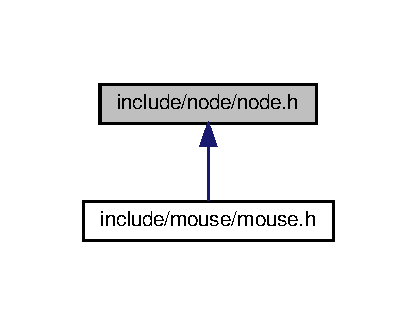
\includegraphics[width=200pt]{node_8h__dep__incl}
\end{center}
\end{figure}
\subsection*{Classes}
\begin{DoxyCompactItemize}
\item 
class \hyperlink{classrwa2_1_1_node}{rwa2\+::\+Node}
\begin{DoxyCompactList}\small\item\em Class to represent a node (cell) in a maze. \end{DoxyCompactList}\end{DoxyCompactItemize}


\subsection{Detailed Description}
This file contains a class to represent a node in a maze. 

\begin{DoxyAuthor}{Author}
Ninad Harishchandrakar (\href{mailto:ninadh@umd.edu}{\tt ninadh@umd.\+edu}) 
\end{DoxyAuthor}
\begin{DoxyVersion}{Version}
0.\+1 
\end{DoxyVersion}
\begin{DoxyDate}{Date}
2021-\/11-\/15
\end{DoxyDate}
\begin{DoxyCopyright}{Copyright}
Copyright (c) 2021 
\end{DoxyCopyright}

\hypertarget{util_8h}{}\section{include/util/util.h File Reference}
\label{util_8h}\index{include/util/util.\+h@{include/util/util.\+h}}


Components used by multiple classes but not required to be a class member can be placed in this file.  


This graph shows which files directly or indirectly include this file\+:\nopagebreak
\begin{figure}[H]
\begin{center}
\leavevmode
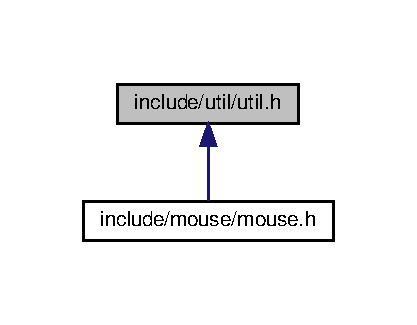
\includegraphics[width=200pt]{util_8h__dep__incl}
\end{center}
\end{figure}
\subsection*{Enumerations}
\begin{DoxyCompactItemize}
\item 
enum \hyperlink{util_8h_a99f26e6ee9fcd62f75203b5402df8098}{direction} \{ \hyperlink{util_8h_a99f26e6ee9fcd62f75203b5402df8098ad0611de6f28d4a9c9eac959f5344698e}{N\+O\+R\+TH} = 0, 
\hyperlink{util_8h_a99f26e6ee9fcd62f75203b5402df8098ab5b3793b961949c817c7c0d99c05dad7}{E\+A\+ST} = 1, 
\hyperlink{util_8h_a99f26e6ee9fcd62f75203b5402df8098a8ef5c0bce69283a9986011a63eea8a6b}{S\+O\+U\+TH} = 2, 
\hyperlink{util_8h_a99f26e6ee9fcd62f75203b5402df8098ae9449e8683a8199dad36b07a63b2f523}{W\+E\+ST} = 3
 \}\begin{DoxyCompactList}\small\item\em Definition of an enum to store the different directions. \end{DoxyCompactList}
\end{DoxyCompactItemize}


\subsection{Detailed Description}
Components used by multiple classes but not required to be a class member can be placed in this file. 

\begin{DoxyAuthor}{Author}
Zeid Kootbally (\href{mailto:zeidk@umd.edu}{\tt zeidk@umd.\+edu}) 
\end{DoxyAuthor}
\begin{DoxyVersion}{Version}
0.\+1 
\end{DoxyVersion}
\begin{DoxyDate}{Date}
2021-\/10-\/24
\end{DoxyDate}
\begin{DoxyCopyright}{Copyright}
Copyright (c) 2021 
\end{DoxyCopyright}


\subsection{Enumeration Type Documentation}
\mbox{\Hypertarget{util_8h_a99f26e6ee9fcd62f75203b5402df8098}\label{util_8h_a99f26e6ee9fcd62f75203b5402df8098}} 
\index{util.\+h@{util.\+h}!direction@{direction}}
\index{direction@{direction}!util.\+h@{util.\+h}}
\subsubsection{\texorpdfstring{direction}{direction}}
{\footnotesize\ttfamily enum \hyperlink{util_8h_a99f26e6ee9fcd62f75203b5402df8098}{direction}}



Definition of an enum to store the different directions. 

\begin{DoxyEnumFields}{Enumerator}
\raisebox{\heightof{T}}[0pt][0pt]{\index{N\+O\+R\+TH@{N\+O\+R\+TH}!util.\+h@{util.\+h}}\index{util.\+h@{util.\+h}!N\+O\+R\+TH@{N\+O\+R\+TH}}}\mbox{\Hypertarget{util_8h_a99f26e6ee9fcd62f75203b5402df8098ad0611de6f28d4a9c9eac959f5344698e}\label{util_8h_a99f26e6ee9fcd62f75203b5402df8098ad0611de6f28d4a9c9eac959f5344698e}} 
N\+O\+R\+TH&North direction \\
\hline

\raisebox{\heightof{T}}[0pt][0pt]{\index{E\+A\+ST@{E\+A\+ST}!util.\+h@{util.\+h}}\index{util.\+h@{util.\+h}!E\+A\+ST@{E\+A\+ST}}}\mbox{\Hypertarget{util_8h_a99f26e6ee9fcd62f75203b5402df8098ab5b3793b961949c817c7c0d99c05dad7}\label{util_8h_a99f26e6ee9fcd62f75203b5402df8098ab5b3793b961949c817c7c0d99c05dad7}} 
E\+A\+ST&East direction \\
\hline

\raisebox{\heightof{T}}[0pt][0pt]{\index{S\+O\+U\+TH@{S\+O\+U\+TH}!util.\+h@{util.\+h}}\index{util.\+h@{util.\+h}!S\+O\+U\+TH@{S\+O\+U\+TH}}}\mbox{\Hypertarget{util_8h_a99f26e6ee9fcd62f75203b5402df8098a8ef5c0bce69283a9986011a63eea8a6b}\label{util_8h_a99f26e6ee9fcd62f75203b5402df8098a8ef5c0bce69283a9986011a63eea8a6b}} 
S\+O\+U\+TH&South direction \\
\hline

\raisebox{\heightof{T}}[0pt][0pt]{\index{W\+E\+ST@{W\+E\+ST}!util.\+h@{util.\+h}}\index{util.\+h@{util.\+h}!W\+E\+ST@{W\+E\+ST}}}\mbox{\Hypertarget{util_8h_a99f26e6ee9fcd62f75203b5402df8098ae9449e8683a8199dad36b07a63b2f523}\label{util_8h_a99f26e6ee9fcd62f75203b5402df8098ae9449e8683a8199dad36b07a63b2f523}} 
W\+E\+ST&West direction \\
\hline

\end{DoxyEnumFields}

%--- End generated contents ---

% Index
\backmatter
\newpage
\phantomsection
\clearemptydoublepage
\addcontentsline{toc}{chapter}{Index}
\printindex

\end{document}
